\section{Database Schema Design}\chapter{Database Schema}

\label{sec:schema}\label{ch:database-schema}



\subsection{Schema Diagram}\section{Schema Overview}

\label{sec:schema-overview}

\begin{figure}[H]

\centeringThis chapter provides the complete SQL schema definition for \projectname{}, including all tables, columns, data types, constraints, and indexes.

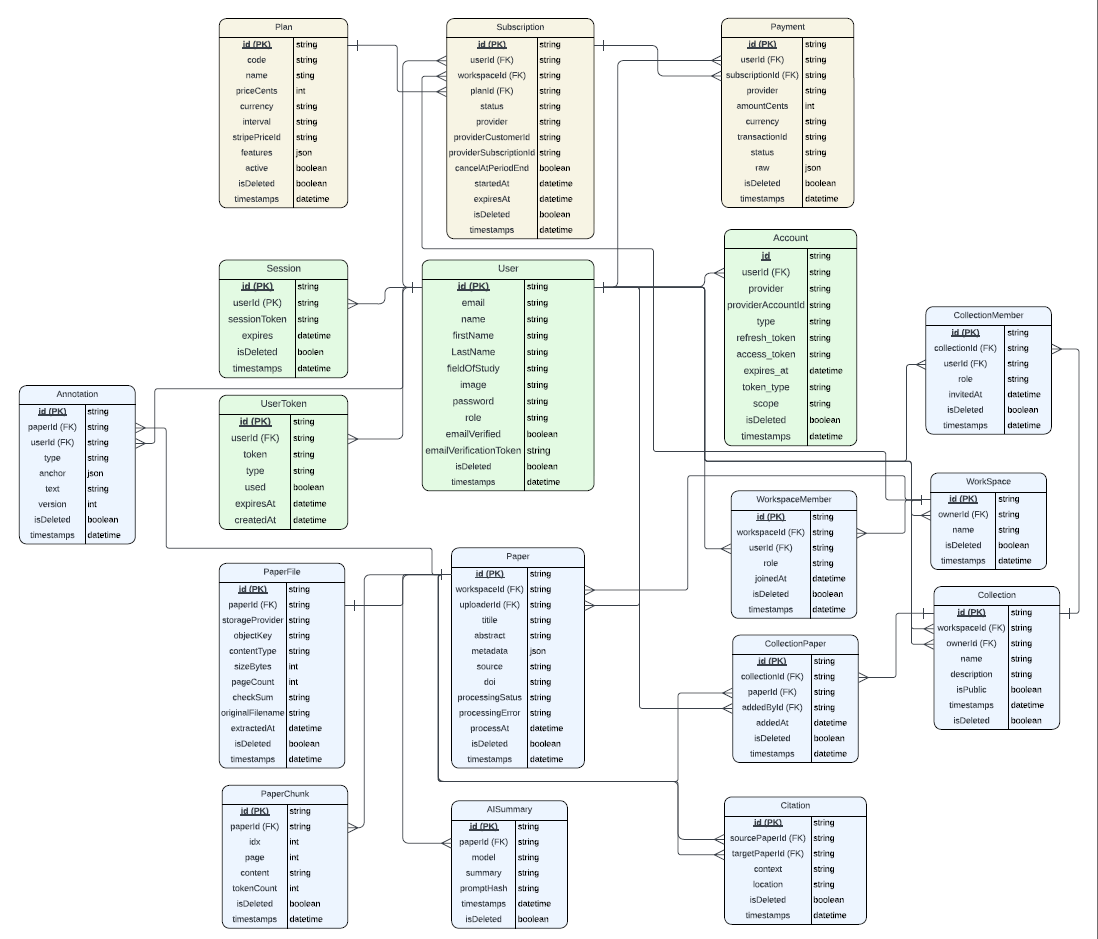
\includegraphics[width=0.95\textwidth]{images/diagrams/schema.png}

\caption{Complete Database Schema with Relationships}% ============================================

\label{fig:schema}% SCHEMA DIAGRAM

\end{figure}% ============================================

\section{Visual Schema Diagram}

\subsection{Core Tables Overview}\label{sec:schema-diagram}



The database consists of 20 interconnected tables organized into 5 functional modules:\begin{figure}[H]

\centering

\textbf{1. Authentication \& User Management}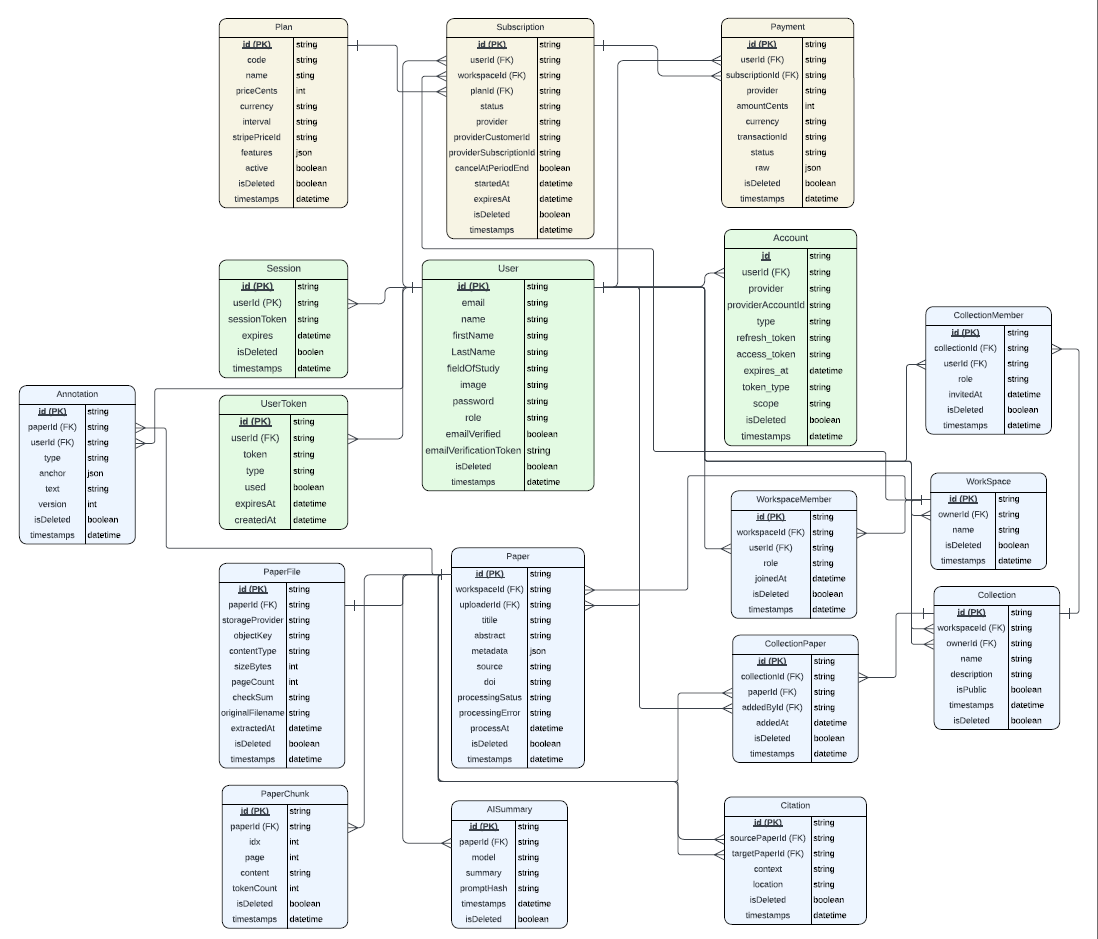
\includegraphics[width=0.95\textwidth]{images/diagrams/schema.png}

\begin{itemize}[leftmargin=*,topsep=3pt,itemsep=2pt]\caption{ScholarFlow Complete Database Schema}

    \item \texttt{User}: User profiles with authentication credentials (email, password hash)\label{fig:schema-complete}

    \item \texttt{Account}: OAuth provider accounts linked to users (Google, GitHub)\end{figure}

    \item \texttt{Session}: Active user sessions with JWT tokens

    \item \texttt{VerificationToken}: Email verification and password reset tokens\noindent For detailed schema view: \url{https://lucid.app/lucidchart/8fa45201-ebc1-46e2-8204-93c162cbaf0b}

\end{itemize}

% ============================================

\textbf{2. Paper Management}% TABLE DEFINITIONS

\begin{itemize}[leftmargin=*,topsep=3pt,itemsep=2pt]% ============================================

    \item \texttt{Paper}: Research papers with metadata (title, authors, abstract, publication year)\section{Core Table Definitions}

    \item \texttt{PaperFile}: File storage references (S3 URLs, file sizes, MIME types)\label{sec:schema-tables}

    \item \texttt{PaperChunk}: Text segments extracted from papers for AI processing

    \item \texttt{PaperTag}: Custom tags for categorization\subsection{User Table}

\end{itemize}

\begin{lstlisting}[language=SQL, caption={User Table Schema}]

\textbf{3. Collections \& Organization}CREATE TABLE "User" (

\begin{itemize}[leftmargin=*,topsep=3pt,itemsep=2pt]  id SERIAL PRIMARY KEY,

    \item \texttt{Collection}: User-created collections with privacy settings  name VARCHAR(255),

    \item \texttt{CollectionPaper}: Many-to-many relationship between collections and papers  email VARCHAR(255) UNIQUE NOT NULL,

    \item \texttt{CollectionMember}: Shared collection access with role-based permissions  emailVerified TIMESTAMP,

\end{itemize}  image TEXT,

  password TEXT,

\textbf{4. AI Features}  role VARCHAR(50) DEFAULT 'RESEARCHER',

\begin{itemize}[leftmargin=*,topsep=3pt,itemsep=2pt]  bio TEXT,

    \item \texttt{AISummary}: AI-generated paper summaries with model metadata  institution VARCHAR(255),

    \item \texttt{AIInsightThread}: Chat conversation threads for paper discussions  field VARCHAR(255),

    \item \texttt{AIInsightMessage}: Individual messages within chat threads  googleScholarUrl TEXT,

\end{itemize}  orcidUrl TEXT,

  createdAt TIMESTAMP DEFAULT NOW(),

\textbf{5. Workspace Collaboration}  updatedAt TIMESTAMP DEFAULT NOW()

\begin{itemize}[leftmargin=*,topsep=3pt,itemsep=2pt]);

    \item \texttt{Workspace}: Team workspaces for collaborative research

    \item \texttt{WorkspaceMember}: Members with roles (RESEARCHER, TEAM\_LEAD, OWNER)-- Indexes

    \item \texttt{WorkspaceInvitation}: Pending workspace invitationsCREATE UNIQUE INDEX "User_email_key" ON "User"(email);

\end{itemize}CREATE INDEX "User_role_idx" ON "User"(role);

\end{lstlisting}

\textbf{6. Subscription \& Billing}

\begin{itemize}[leftmargin=*,topsep=3pt,itemsep=2pt]\subsection{Paper Table}

    \item \texttt{Subscription}: User subscription plans (FREE, PRO, INSTITUTIONAL)

    \item \texttt{Payment}: Payment transaction history with Stripe integration\begin{lstlisting}[language=SQL, caption={Paper Table Schema}]

    \item \texttt{UsageEvent}: API usage tracking for rate limiting and billingCREATE TABLE "Paper" (

\end{itemize}  id SERIAL PRIMARY KEY,

  title VARCHAR(500) NOT NULL,

\subsection{Key Relationships}  authors TEXT,

  abstract TEXT,

\begin{itemize}[leftmargin=*,topsep=3pt,itemsep=2pt]  publicationYear INTEGER,

    \item \textbf{User $\to$ Paper}: One-to-many (users upload multiple papers)  journal VARCHAR(255),

    \item \textbf{Paper $\to$ Collection}: Many-to-many via \texttt{CollectionPaper}  doi VARCHAR(255),

    \item \textbf{User $\to$ Workspace}: Many-to-many via \texttt{WorkspaceMember}  fileUrl TEXT NOT NULL,

    \item \textbf{Paper $\to$ AISummary}: One-to-many (multiple AI summaries per paper)  fileName VARCHAR(500) NOT NULL,

    \item \textbf{Paper $\to$ AIInsightThread}: One-to-many (chat threads per paper)  fileSize BIGINT NOT NULL,

    \item \textbf{User $\to$ Subscription}: One-to-one (each user has one active subscription)  fileType VARCHAR(50) NOT NULL,

\end{itemize}  uploaderId INTEGER NOT NULL REFERENCES "User"(id),

  workspaceId INTEGER NOT NULL REFERENCES "Workspace"(id),

\subsection{Data Types \& Constraints}  isDeleted BOOLEAN DEFAULT FALSE,

  deletedAt TIMESTAMP,

\begin{itemize}[leftmargin=*,topsep=3pt,itemsep=2pt]  createdAt TIMESTAMP DEFAULT NOW(),

    \item \textbf{Primary Keys}: UUID (universally unique identifiers) for all tables  updatedAt TIMESTAMP DEFAULT NOW()

    \item \textbf{Foreign Keys}: Cascading deletes where appropriate (e.g., deleting user deletes sessions));

    \item \textbf{Unique Constraints}: Email addresses, OAuth provider accounts

    \item \textbf{Nullable Fields}: Optional metadata (publication year, DOI, journal)-- Performance Indexes

    \item \textbf{Timestamps}: \texttt{createdAt} and \texttt{updatedAt} on all tablesCREATE INDEX "Paper_uploaderId_workspaceId_idx" 

    \item \textbf{Soft Deletes}: \texttt{isDeleted} flag for papers and collections  ON "Paper"(uploaderId, workspaceId);

\end{itemize}CREATE INDEX "Paper_workspaceId_isDeleted_idx" 

  ON "Paper"(workspaceId, isDeleted);

\subsection{Indexing Strategy}CREATE INDEX "Paper_title_authors_gin_idx" 

  ON "Paper" USING gin(to_tsvector('english', title || ' ' || authors));

\begin{itemize}[leftmargin=*,topsep=3pt,itemsep=2pt]\end{lstlisting}

    \item \textbf{Unique Indexes}: \texttt{User.email}, \texttt{Account.(provider, providerAccountId)}

    \item \textbf{Foreign Key Indexes}: All foreign key columns for efficient joins% NOTE: Additional tables should be added here

    \item \textbf{Composite Indexes}: \texttt{(workspaceId, uploaderId)}, \texttt{(collectionId, paperId)}% See apps/backend/prisma/schema.prisma for complete definitions

    \item \textbf{Full-Text Indexes}: \texttt{Paper.title}, \texttt{Paper.abstract} for search% Key tables to include:

    \item \textbf{Timestamp Indexes}: \texttt{createdAt} columns for chronological queries% - Workspace

\end{itemize}% - Collection

% - AISummary
% - Subscription
% - Annotation
% - CitationExport
% etc.

\section{Complete Schema SQL}
\label{sec:schema-complete-sql}

\begin{infobox}[Full Schema]
The complete schema includes 24 tables with all relationships. For the full Prisma schema definition, see:

\texttt{apps/backend/prisma/schema.prisma}

Or generate SQL:
\begin{lstlisting}[language=bash]
yarn db:migrate dev --name schema_export
\end{lstlisting}
\end{infobox}
